\documentclass[12pt]{article}
\usepackage{lecture}
\usepackage{graphicx}
\usepackage{epstopdf}
\usepackage{html}
\usepackage{url}

\newcommand{\copyrightYears}{2001-2021}

\title{Detecting selection on nucleotide polymorphisms}

\begin{document}

\maketitle

\thispagestyle{first}

\section*{Introduction}

At this point, we've refined the neutral theory quite a bit. Our
understanding of how molecules evolve now recognizes that some
substitutions are more likely than others, but we're still proceeding
under the assumption that most nucleotide substitutions are neutral or
detrimental. So far we've argued that variation like what Hubby and
Lewontin~\cite{Hubby-Lewontin66,Lewontin-Hubby66} found is not likely
to be maintained by natural selection. But we have strong evidence
that heterozygotes for the sickle-cell allele are more fit than either
homozygote in human populations where malaria is prevalent. That's an
example where selection is acting to maintain a polymorphism, not to
eliminate it. Are there other examples? How could we detect them?

In the 1970s a variety of studies suggested that a polymorphism in the
locus coding for alcohol dehydrogenase in {\it Drosophila
  melanogaster\/} might not only be subject to selection but that
selection may be acting to maintain the polymorphism. As DNA
sequencing became more practical at about the same time,\footnote{It
  was still {\it vastly\/} more laborious than it is now.} population
geneticists began to realize that comparative analyses of DNA
sequences at protein-coding loci could provide a powerful tool for
unraveling the action of natural selection. Synonymous sites within a
protein-coding sequence provide a powerful standard of
comparison. Regardless of

\begin{itemize}

\item the demographic history of the population from which the
  sequences were collected,

\item the length of time that populations have been evolving under the
  sample conditions and whether it has been long enough for the
  population to have reached a drift-migration-mutation-selection
  equilibrium, or

\item the actual magnitude of the mutation rate, the migration rate,
  or the selection coefficients

\end{itemize}

\noindent the synonymous positions within the sequence provide an
internal control on the amount and pattern of differentiation that
should be expected when substitutions are neutral.\footnote{Ignoring,
  for the moment, the possibility that there may be selection on codon
  usage.}  Thus, if we see different patterns of nucleotide
substitution at synonymous and non-synonymous sites, we can infer that
selection is having an effect on amino acid substitutions.

\section*{Nucleotide sequence variation at the {\it Adh\/} locus in
  {\it Drosophila melanogaster}}\index{Drosophila@\textit{Drosophila}!\textit{melanogaster}}\index{alcohol dehydrogenase}\index{Adh}

Kreitman~\cite{Kreitman83} took advantage of these ideas to provide
additional insight into whether natural selection was likely to be
involved in maintaining the polymorphism at {\it Adh\/} in {\it
  Drosophila melanogaster}. He cloned and sequenced 11 alleles at this
locus, each a little less than 2.4kb in length.\footnote{Think about
  how the technology has changed since then. This work represented a
  major part of his Ph.D. dissertation, and the results were published
  as an article in {\it Nature}. Now an undergraduate would do
  substantially more for an independent study project.} If we restrict
our attention to the coding region, a total of 765bp, there were 6
distinct sequences that differed from one another at between 1 and 13
sites. Given the observed level of polymorphism within the gene, there
should be 9 or 10 amino acid differences observed as well, but only
one of the nucleotide differences results in an amino acid difference,
the amino acid difference associated with the already recognized
electrophoretic polymorphism. Thus, there is significantly less amino
acid diversity than expected if nucleotide substitutions were neutral,
consistent with my assertion that most mutations are deleterious and
that natural selection will tend to eliminate
them.\index{Adh!purifying selection} In other words, another example
of the ``sledgehammer principle.''\index{sledgehammer principle}

Does this settle the question? Is the {\it Adh\/} polymorphism another
example of allelic variants being neutral or selected against? Would I
be asking these questions if the answer were ``Yes''?

\subsection*{Kreitman and Aguad{\'e}}

A few years after Kreitman~\cite{Kreitman83} appeared, Kreitman and
Aguad{\'e}~\cite{Kreitman-Aguade86} published an analysis in which
they looked at levels of nucleotide diversity in the {\it Adh\/}
region, as revealed through analysis of RFLPs, in {\it
  D. melanogaster\/} and the closely related {\it D. simulans}. Why
the comparative approach? Well, Kreitman and Aguad{\'e} recognized
that the neutral theory of molecular evolution makes two predictions
that are related to the underlying mutation rate:

\begin{itemize}

\item If mutations are neutral, the substitution rate is equal to the
  mutation rate.

\item If mutations are neutral, the diversity within populations
  should be about $4N_e\mu/(4N_e\mu + 1)$.

\end{itemize}

\noindent Thus, if variation at the {\it Adh\/} locus in {\it
  D. melanogaster\/} is selectively neutral, the amount of divergence
between {\it D. melanogaster\/} and {\it D. simulans\/} should be
related to the amount of diversity within each. What they found
instead is summarized in Table~\ref{table:ka}.\index{Adh!balancing selection}\index{diversity-divergence}

The expected level of diversity in each part of the {\it Adh\/} locus
is calculated assuming that the probability of polymorphism is
independent of what position in the locus we are
examining.\footnote{It's important to note that what I've labeled as
  the {\it Adh\/} locus in Table~\ref{table:ka} is the region that
  contains the protein coding part of the locus. The 5' and 3'
  flanking regions are physically adjacent, but none of the
  nucleotides in these parts of the gene are translated into the {\it
    Adh\/} enzyme.} Specifically, Kreitman and Aguad{\'e} calculated
the expected polymorphism as follows:

\begin{itemize}

\item They calculated the number of ``site equivalents'' in each
  region of the locus. A site equivalent is the actual length of the
  region~(in number of nucleotides) times the fraction of changes
  within that sequence that would lead to gain or loss of a
  restriction site.\footnote{Because sequencing was extremely
    time-consuming in the mid-1980s, it was impractical to sequence
    the {\it Adh\/} locus in all of the 81 lines they used in the
    analysis. Instead they used restriction enzymes to reveal some of
    the nucleotide sequence variation in the locus.} There were 414
  site equivalents in the 5' flanking region, 411 site equivalents in
  the {\it Adh\/} locus, and 129 site equivalents in the 3' flanking
  region.

\item They calculated the fraction of site equivalents that were
  polymorphic across the entire locus:
\[
\frac{25}{414+411+129} \approx 0.026 \quad .
\]

\item They calculated the expected number of polymorphic sites within
  a region as the product of the number of site equivalents and the
  fraction of polymorphic site equivalents.

\end{itemize}

\noindent They used the same approach to calculate the expected
divergence between {\it D. melanogaster\/} and {\it D. simulans\/}
with one important exception. They directly compared the nucleotide
sequence of one {\it Adh\/} allele from {\it D. melanogaster\/} with
one {\it Adh\/} allele from {\it D. simulans}.\footnote{Can you
  explain why it's reasonable to estimate divergence between alleles
  in these species using only one allele from each of them?} As a
result, they didn't have to use the site equivalent correction. They
could directly use the number of nucleotides in each region of the
gene.

\begin{table}
\begin{center}
\begin{tabular}{l|ccc}
\hline\hline
         & 5' flanking & {\it Adh\/} locus & 3' flanking \\
\hline
Diversity$^1$ \\
\quad Observed & 9     & {\bf 14}   & 2    \\
\quad Expected & 10.8  & 10.8 & 3.4  \\
Divergence$^2$ \\
\quad Observed & 86    & 48   & 31   \\
\quad Expected & 55    & {\bf 76.9} & 33.1 \\
\hline
\multicolumn{4}{l}{$^1$Number of polymorphic sites within {\it
         D. melanogaster\/}} \\
\multicolumn{4}{l}{$^2$Number of nucleotide differences between {\it
         D. melanogaster\/} and {\it D. simulans}}
\end{tabular}
\end{center}
\caption{Diversity and divergence in the {\it Adh\/} region of {\it
    Drosophila}~(from~\cite{Kreitman-Aguade86}).}\label{table:ka}
\end{table}

Notice that there is substantially less divergence between {\it
  D. melanogaster\/} and {\it D. simulans\/} at the {\it Adh\/} locus
than would be expected, based on the average level of divergence
across the entire region. That's consistent with the earlier
observation that most amino acid substitutions are selected
against. On the other hand, there is {\it more\/} nucleotide diversity
within {\it D. melanogaster\/} than would be expected based on the
levels of diversity seen in across the entire region. What gives?

Time for a trip down memory lane. Remember something called
``coalescent theory?'' It told us that for a sample of neutral genes
from a population, the expected time back to a common ancestor for all
of them is about $4N_e$ for a nuclear gene in a diploid
population. That means there's been about $4N_e$ generations for
mutations to occur. Suppose, however, that the electrophoretic
polymorphism were being maintained by natural selection. Then we might
well expect that it would be maintained for a lot longer than $4N_e$
generations. If so, there would be a lot more time for diversity to
accumulate. Thus, the excess diversity could be accounted for if there
is balancing selection at ADH.\index{coalescent!balancing selection}

\subsection*{Kreitman and Hudson}

Kreitman and Hudson~\cite{Kreitman-Hudson91} extended this approach by
looking more carefully within the region to see where they could find
differences between observed and expected levels of nucleotide
sequence diversity. They used a ``sliding window'' of 100 silent base
pairs in their calculations. By ``sliding window'' what they mean is
that first they calculate statistics for bases 1-100, then for bases
2-101, then for bases 3-102, and so on until they hit the end of the
sequence~(Figure~\ref{fig:kh}).

\begin{figure}
\begin{center}
\resizebox{!}{7cm}{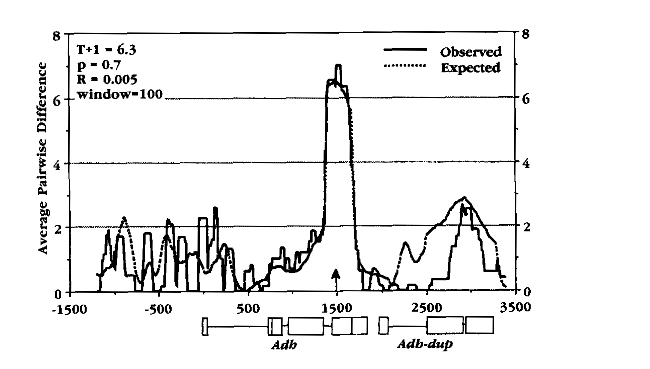
\includegraphics{kreitman-hudson.eps}}
\end{center}
\caption{Sliding window analysis of nucleotide diversity in the {\it
    Adh\/}-{\it Adh-dup} region of {\it Drosophila melanogaster}. The
  arrow marks the position of the single nucleotide substitution that
  distinguishes {\it Adh-F\/} from {\it
    Adh-S\/}~(from~\cite{Kreitman-Hudson91})}\label{fig:kh}
\end{figure}

To me there are two particularly striking things about this
figure. First, the position of the single nucleotide substitution
responsible for the electrophoretic polymorphism is clearly
evident. Second, the excess of polymorphism extends for only a 200-300
nucleotides in each direction. That means that the rate of
recombination {\it within\/} the gene is high enough to randomize the
nucleotide sequence variation farther away.\footnote{Remember this
  observation when we get to association mapping at the end of the
  course. In organisms with a large effective population size,
  associations due to physical linkage may fall off {\it very\/}
  rapidly, meaning that you would have to have a {\it very\/} dense
  map to have a hope of finding associations.}

\section*{Detecting selection in the human genome}

I've already mentioned the HapMap project~\cite{HapMap-2007}, a
collection of genotype data at roughly 3.2M SNPs in the human
genome. The data in phase II of the project were collected from four
populations:

\begin{itemize}

\item Yoruba (Ibadan, Nigeria)

\item Japanese (Tokyo, Japan)

\item Han Chinese (Beijing, China)

\item ancestry from northern and western Europe (Utah, USA)

\end{itemize}

We expect genetic drift to result in allele frequency differences
among populations, and we can summarize the extent of that
differentiation at each locus with $F_{ST}$. If all HapMap SNPs are
selectively neutral,\footnote{And unlinked to sites that are under
  selection.} then all loci should have the same $F_{ST}$ within the
bounds of statistical sampling error and the evolutionary sampling due
to genetic drift. A scan of human chromosome 7 reveals both a lot of
variation in individual-locus estimates of $F_{ST}$ and a number of
loci where there is substantially more differentiation among
populations than is expected by
chance~(Figure~\ref{fig:low-res-SNP}). At very fine genomic scales we
can detect even more outliers~(Figure~\ref{fig:high-res-SNP}),
suggesting that human populations have been subject to divergent
selection pressures at many different loci~\cite{Guo-etal-2009}.\index{F-statistics@$F$-statistics!outliers}

\begin{figure}
\begin{center}
\resizebox{\textwidth}{!}{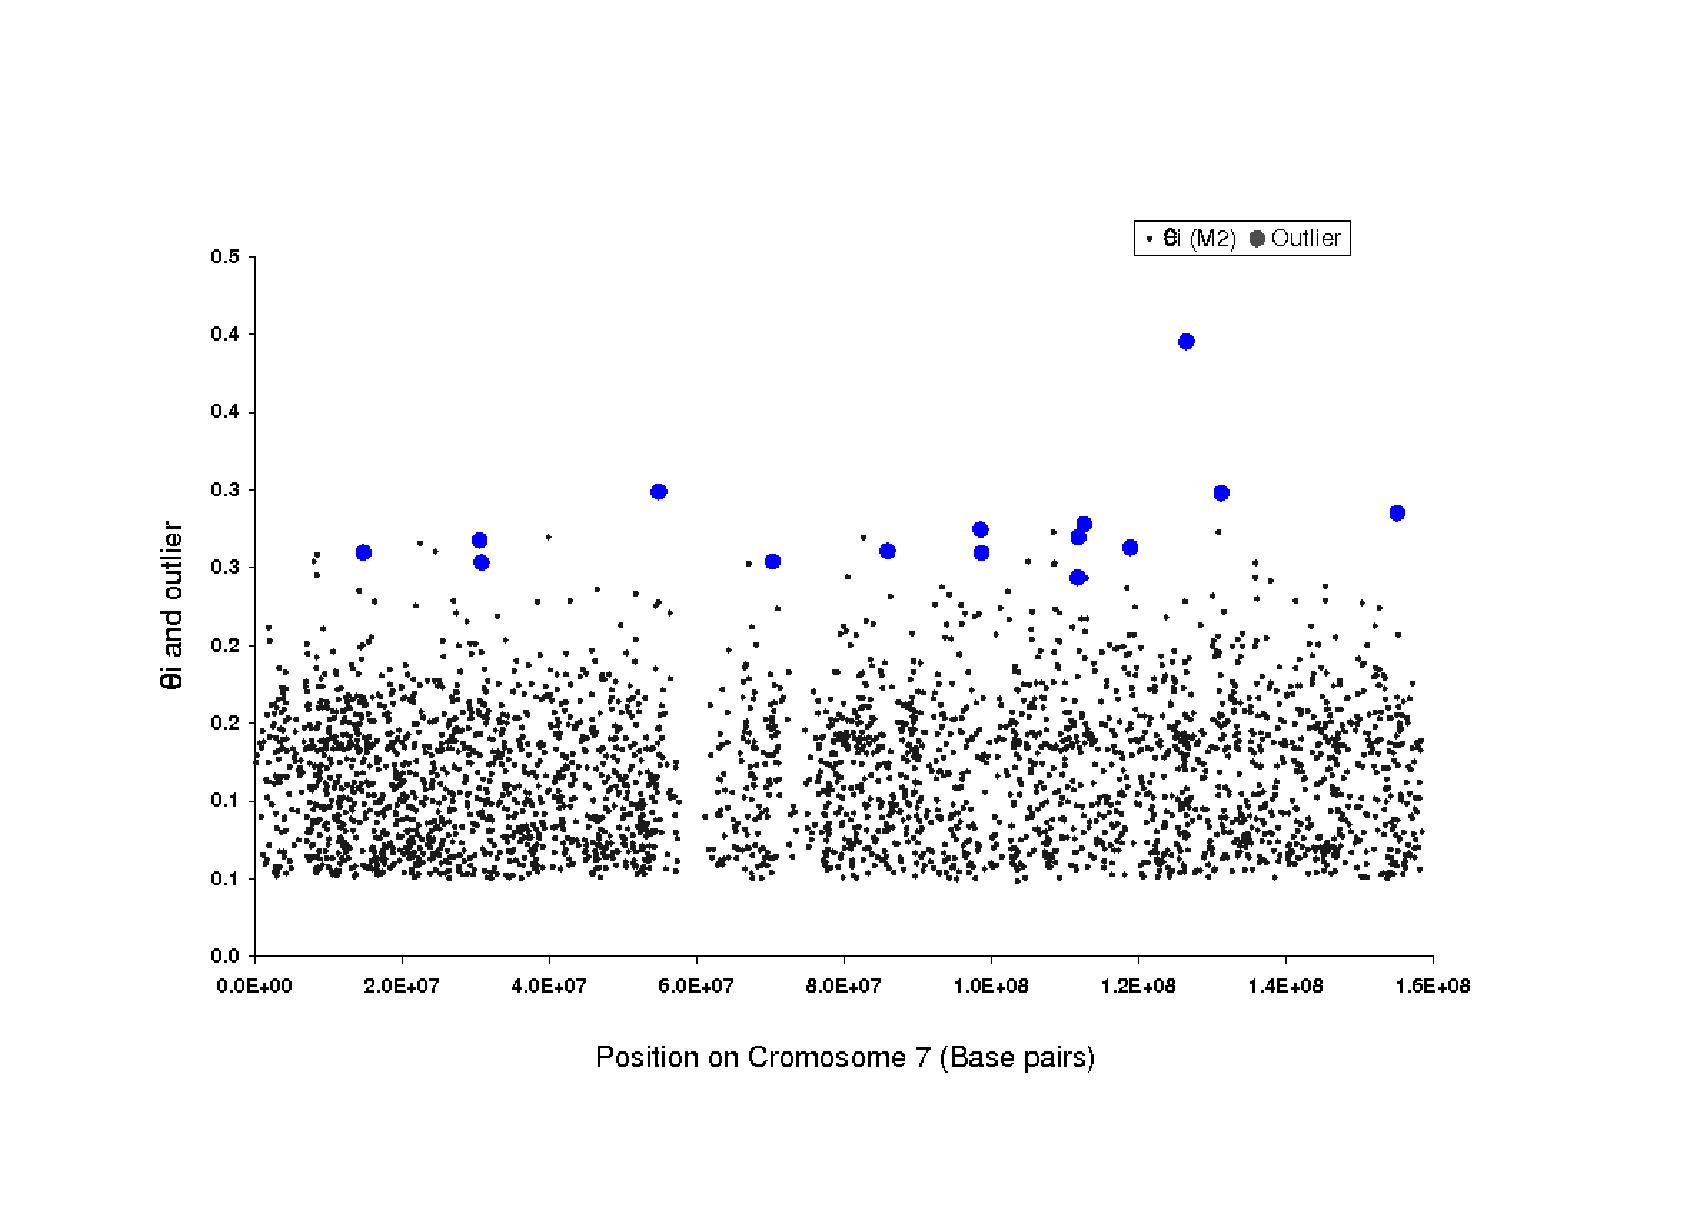
\includegraphics{outlier.eps}}
\end{center}
\caption{Single-locus estimates of $F_{ST}$ along chromosome 7 in the
  HapMap data set. Blue dots denote outliers. Adjacent SNPs in this
  sample are separated, on average, by about
  52kb. (from~\cite{Guo-etal-2009})}\label{fig:low-res-SNP}
\end{figure}

\begin{figure}
\begin{center}
\resizebox{0.7\textwidth}{!}{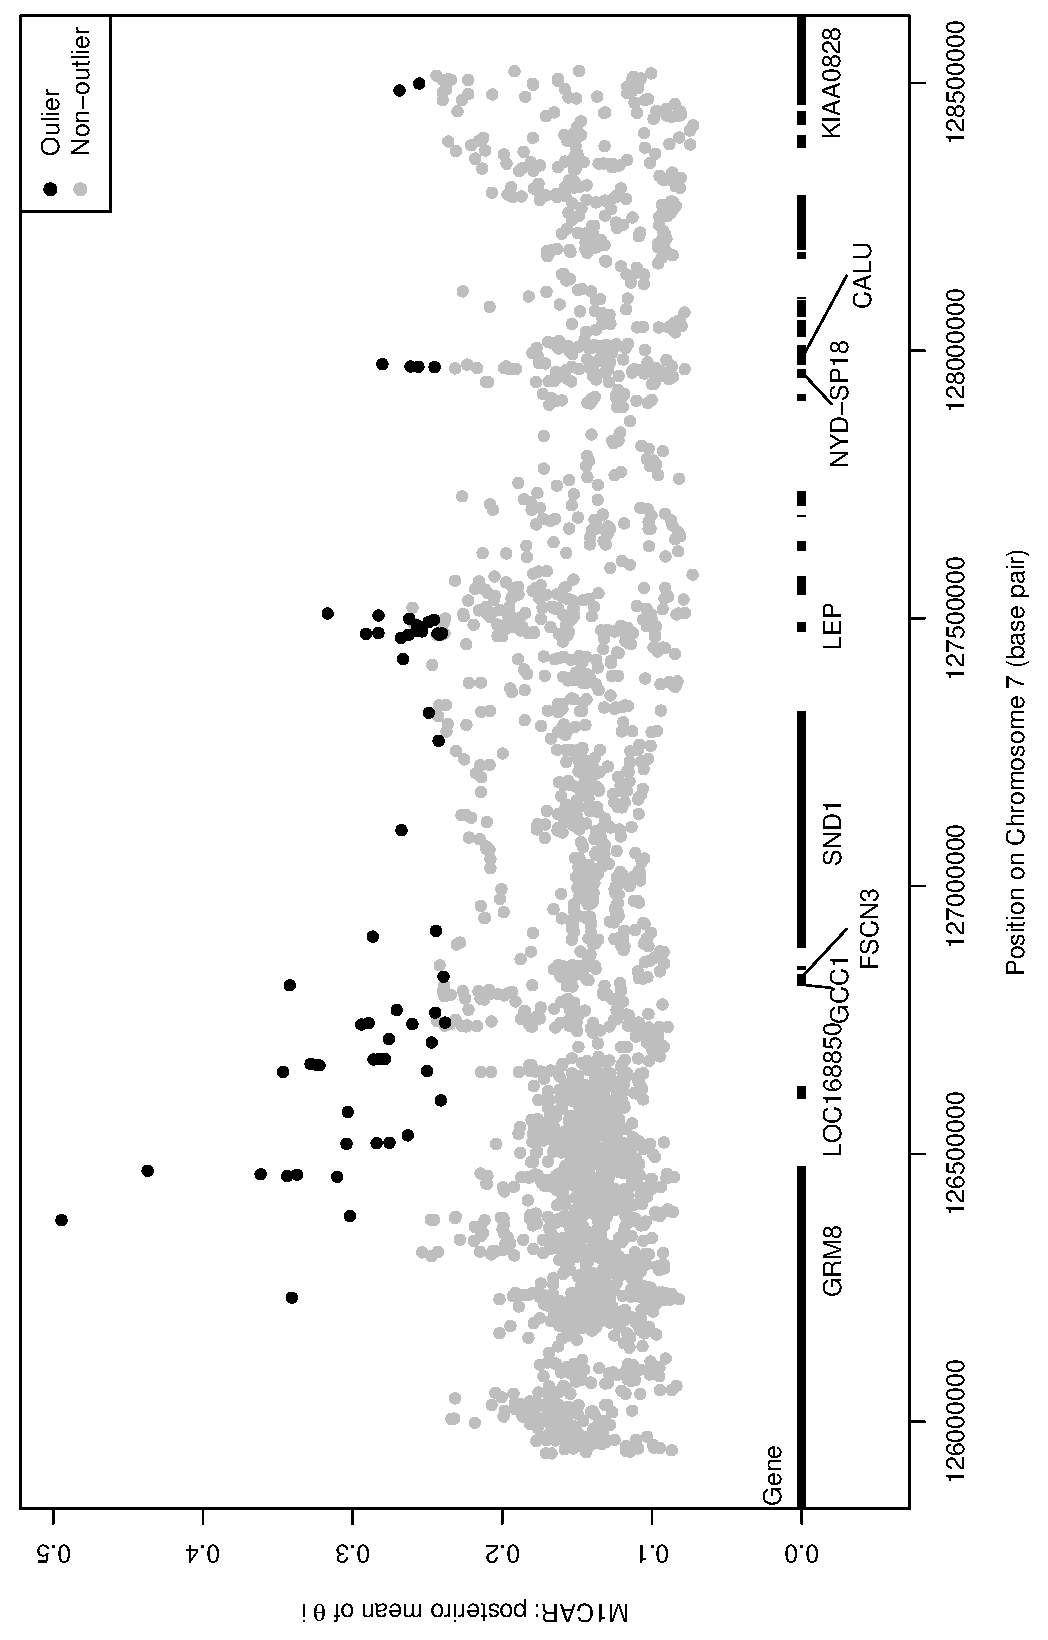
\includegraphics[angle=270]{outlier-high.eps}}
\end{center}
\caption{Single-locus estimates of $F_{ST}$ along a portion of
  chromosome 7 in the HapMap data set. Black dots denote
  outliers. Solid bars refer to previously identified genes. Adjacent
  SNPs in this sample are separated, on average, by about
  1kb. (from~\cite{Guo-etal-2009})}\label{fig:high-res-SNP}
\end{figure}

\section*{Tajima's $D$}\index{Tajima's $D$}

So far we've been comparing rates of synonymous and non-synonymous
substitution to detect the effects of natural selection on molecular
polymorphisms. Tajima~\cite{Tajima89} proposed a method that builds on
the foundation of the neutral theory of molecular evolution in a
different way. I've already mentioned the infinite alleles model of
mutation several times. When thinking about DNA sequences a closely
related approximation is to imagine that every time a mutation occurs,
it occurs at a different site.\footnote{Of course, we know this isn't
  true. Multiple substitutions {\it can\/} occur at any site. That's
  why the percent difference between two sequences isn't equal to the
  number of substitutions that have happened at any particular
  site. We're simply assuming that the sequences we're comparing are
  closely enough related that nearly all mutations have occurred at
  different positions.} If we do that, we have an {\it infinite
  sites\/} model of mutation.\index{mutation!infinite sites model}

When dealing with nucleotide sequences in a population context there
are two statistics of potential interest:

\begin{itemize}

\item The {\it number\/} of nucleotide positions at which a
  polymorphism is found or, equivalently, the number of segregating
  sites, $k$.\index{segregating sites}

\item The average number of nucleotide differences between two
  sequences, $\pi$, where $\pi$ is estimated as\index{nucleotide diversity}
\[
\pi = \sum x_ix_j\delta_{ij} \quad .
\]
In this expression, $x_i$ is the frequency of the $i$th haplotype and
$\delta_{ij}$ is the number of nucleotide sequence differences between
haplotypes $i$ and $j$.\footnote{I lied, but you must be getting used
  to that by now. This isn't quite the way you estimate it. To get an
  unbiased estimate of $\pi$, you have to multiply this equation by
  $n/(n-1)$, where $n$ is the number of haplotypes in your
  sample. And, of course, if you're Bayesian you'll be even a little
  more careful. You'll estimate $x_i$ using an appropriate prior on
  haplotype frequencies and you'll estimate the probability that
  haplotypes $i$ and $j$ are different at a randomly chosen position
  given the observed number of differences and the sequence length and
  multiply that probability by the sequence length giving you the
  expected number of differences between those two haplotypes. The
  expected number of differences will be close $\delta_{ij}$, but it
  won't be identical and it won't be a single number.}

\end{itemize}

The quantity $4N_e\mu$ comes up a lot in mathematical analyses of
molecular evolution. Population geneticists, being a lazy bunch, get
tired of writing that down all the time, so they invented the
parameter $\theta = 4N_e\mu$ to save themselves a little
time.\footnote{This is {\it not\/} the same $\theta$ we encountered
  when discussing $F$-statistics. Weir and Cockerham's $\theta$ is a
  different beast. I know it's confusing, but that's the way it
  is. When reading a paper, the context should make it clear which
  conception of $\theta$ is being used. Another thing to be careful of
  is that sometimes authors think of $\theta$ in terms of a haploid
  population. When they do, it's $2N_e\mu$. Usually the context makes
  it clear which definition is being used, but you have to remember to
  pay attention to be sure. If you follow population geneticists on
  Twitter, you'll often see them complaining about ``off by two''
  errors.} Under the infinite-sites model of DNA sequence evolution,
it can be shown that
\begin{eqnarray*}
\E(\pi) &=& \theta \\
\E(k) &=& \theta\sum_i^{n-1} \frac{1}{i} \quad ,
\end{eqnarray*}
where $n$ is the number of haplotypes in your sample.\footnote{The
  ``E'' refers to expectation. It is the average value of a random
  variable. $\mbox{E}(\pi)$ is read as ``the expectation of $\pi$.''}
This suggests that there are two ways to estimate $\theta$, namely
\begin{eqnarray*}
\hat \theta_\pi &=& \hat \pi \\
\hat \theta_k   &=& \frac{k}{\sum_i^{n-1}\frac{1}{i}} \quad ,
\end{eqnarray*}
where $\hat\pi$ is the average heterozygosity at nucleotide sites in
our sample and $k$ is the observed number of segregating sites in our
sample.\footnote{If your memory is really good, you may recognize that
  those estimates are method of moments estimates, i.e., parameter
  estimates obtained by equating sample statistics with their expected
  values.} If the nucleotide sequence variation among our haplotypes
is neutral and the population from which we sampled is in equilibrium
with respect to drift and mutation, then $\hat\theta_\pi$ and
$\hat\theta_k$ should be statistically indistinguishable from one
another. In other words,
\[
\hat D = \frac{\hat\theta_\pi -
  \hat\theta_k}{\mbox{Var}(\hat\theta_\pi - \hat\theta_k)} 
\]
should be indistinguishable from zero.\footnote{Dividing the
  difference between $\hat\theta_\pi$ and $\hat\theta_k$ by its
  variance makes the expectation of $\hat D$ zero and gives it a
  variance of one. This allows us to construct a statistical test of
  the difference between the observed $\hat D$ and the expectation if
  sequences are evolving neutrally and if the population is at a
  drift-mutation equilibrium. See~\cite{Tajima89} for details.} If it
is either negative or positive, we can infer that there's some
departure from the assumptions of neutrality and/or equilibrium. Thus,
$\hat D$ can be used as a test statistic to assess whether the data
are consistent with the population being at a neutral mutation-drift
equilibrium. Consider the value of $D$ under following
scenarios:\index{Tajima's $D$!interpretation}

\begin{description}

\item[Neutral variation] If the variation is neutral and the
  population is at a drift-mutation equilibrium, then $\hat D$ will be
  statistically indistinguishable from zero.

\item[Overdominant selection] Overdominance will allow alleles
  belonging to the different classes to become quite divergent from one
  another. $\delta_{ij}$ within each class will be small, but
  $\delta_{ij}$ between classes will be large and both classes will be
  in intermediate frequency, leading to large values of
  $\theta_\pi$. There won't be a similar tendency for the {\it
  number\/} of segregating sites to increase, so $\theta_k$ will be
  relatively unaffected. As a result, $\hat D$ will be positive.

\item[Population bottleneck] If the population has recently undergone
  a bottleneck, then $\pi$ will be little affected unless the
  bottleneck was prolonged and severe.\footnote{Why? Because most of
    the heterozygosity is due to alleles of moderate to high
    frequency, and those are not the ones likely to be lost in a
    bottleneck.}  $k$, however, may be substantially reduced. Thus,
  $\hat D$ should be positive.

\item[Purifying selection] If there is purifying selection, mutations
  will occur and accumulate at silent sites, but they aren't likely
  ever to become very common. Thus, there are likely to be lots of
  segregating sites, but not much heterozygosity, meaning that
  $\hat\theta_k$ will be large, $\hat\theta_\pi$ will be small, and
  $\hat D$ will be negative.

\item[Population expansion] Similarly, if the population has recently
  begun to expand, mutations that occur are unlikely to be lost,
  increasing $\hat\theta_k$, but it will take a long time before they
  contribute to heterozygosity, $\hat\theta_\pi$. Thus, $\hat D$ will
  be negative.

\end{description}

In short, $\hat D$ provides a different avenue for insight into the
evolutionary history of a particular nucleotide sequence. But
interpreting it can be a little tricky.

\begin{description}

\item[$\hat D = 0$:] We have no evidence for changes in population
  size or for any particular pattern of selection at the
  locus.\footnote{Please remember that the failure to detect a difference
    from 0 could mean that your sample size is too small to detect an
    important effect. If you can't detect a difference, you should try
    to assess what values of $D$ are consistent with your data and be
    appropriately circumspect in your conclusions.}

\item[$\hat D < 0$:] The population size may be increasing or we may
  have evidence for purifying selection at this locus.

\item[$\hat D > 0$:] The population may have suffered a recent
  bottleneck (or be decreasing) or we may have evidence for
  overdominant selection at this locus.

\end{description}

\noindent If we have data available for more than one locus, we may be
able to distinguish changes in population size from selection at any
particular locus. After all, all loci will experience the same
demographic effects, but we might expect selection to act differently
at different loci, especially if we choose to analyze loci with
different physiological function.

A quick search in Google Scholar reveals that the paper in which
Tajima described this approach~\cite{Tajima89} has been cited over
13,000
times.\footnote{\url{https://scholar.google.com/scholar?hl=en&as_sdt=0\%2C7&q=tajima+genetics+123\%3A585-595\%3B+1989&btnG=}
  Search on 30 July 2021.} Clearly it has been widely used for
interpreting patterns of nucleotide sequence variation. Although it is
a very useful statistic, Zeng et al.~\cite{Zeng-etal-2006} point out
that there are important aspects of the data that Tajima's $D$ does
not consider. As a result, it may be less powerful, i.e., less able to
detect departures from neutrality, than some alternatives.

% soft sweeps vs. hard sweeps
% Garud (2023)
% Hermisson and Pennings (2005)
% Pennings and Hermisson (2006)

\bibliography{popgen}
\bibliographystyle{plain}

\ccLicense

\end{document}


